%% This is an example first chapter.  You should put chapter/appendix that you
%% write into a separate file, and add a line \include{yourfilename} to
%% main.tex, where `yourfilename.tex' is the name of the chapter/appendix file.
%% You can process specific files by typing their names in at the 
%% \files=
%% prompt when you run the file main.tex through LaTeX.
\chapter{Introduction}

%% Chapter outline goes here
In this chapter, the construction of a fiber optic doppler optical coherence microscopy stem will be motivated. Additionally, the mathematical underpinnings of the system will be introduced, and recent related work will be discussed.

\section{Motivations for a fiber optic DOCM system}

\label{sec:intro}

The mammilian cochlea is capable of remarkable sensory perception. It can distinguish vibratory motion as small as the radius of a hydrogen atom and discriminate between up to 30 frequencies within a single semitone. \cite{ghafarri} However, the mechanics of motion in the inner ear remain poorly understood. The Micromechanics Group at the Research Laboratory of Electronics at MIT is analyzing motion in the cochlea in order to more fully understand what enables these remarkable sensory capabilities.

\begin{figure}[h!]
  \centering
    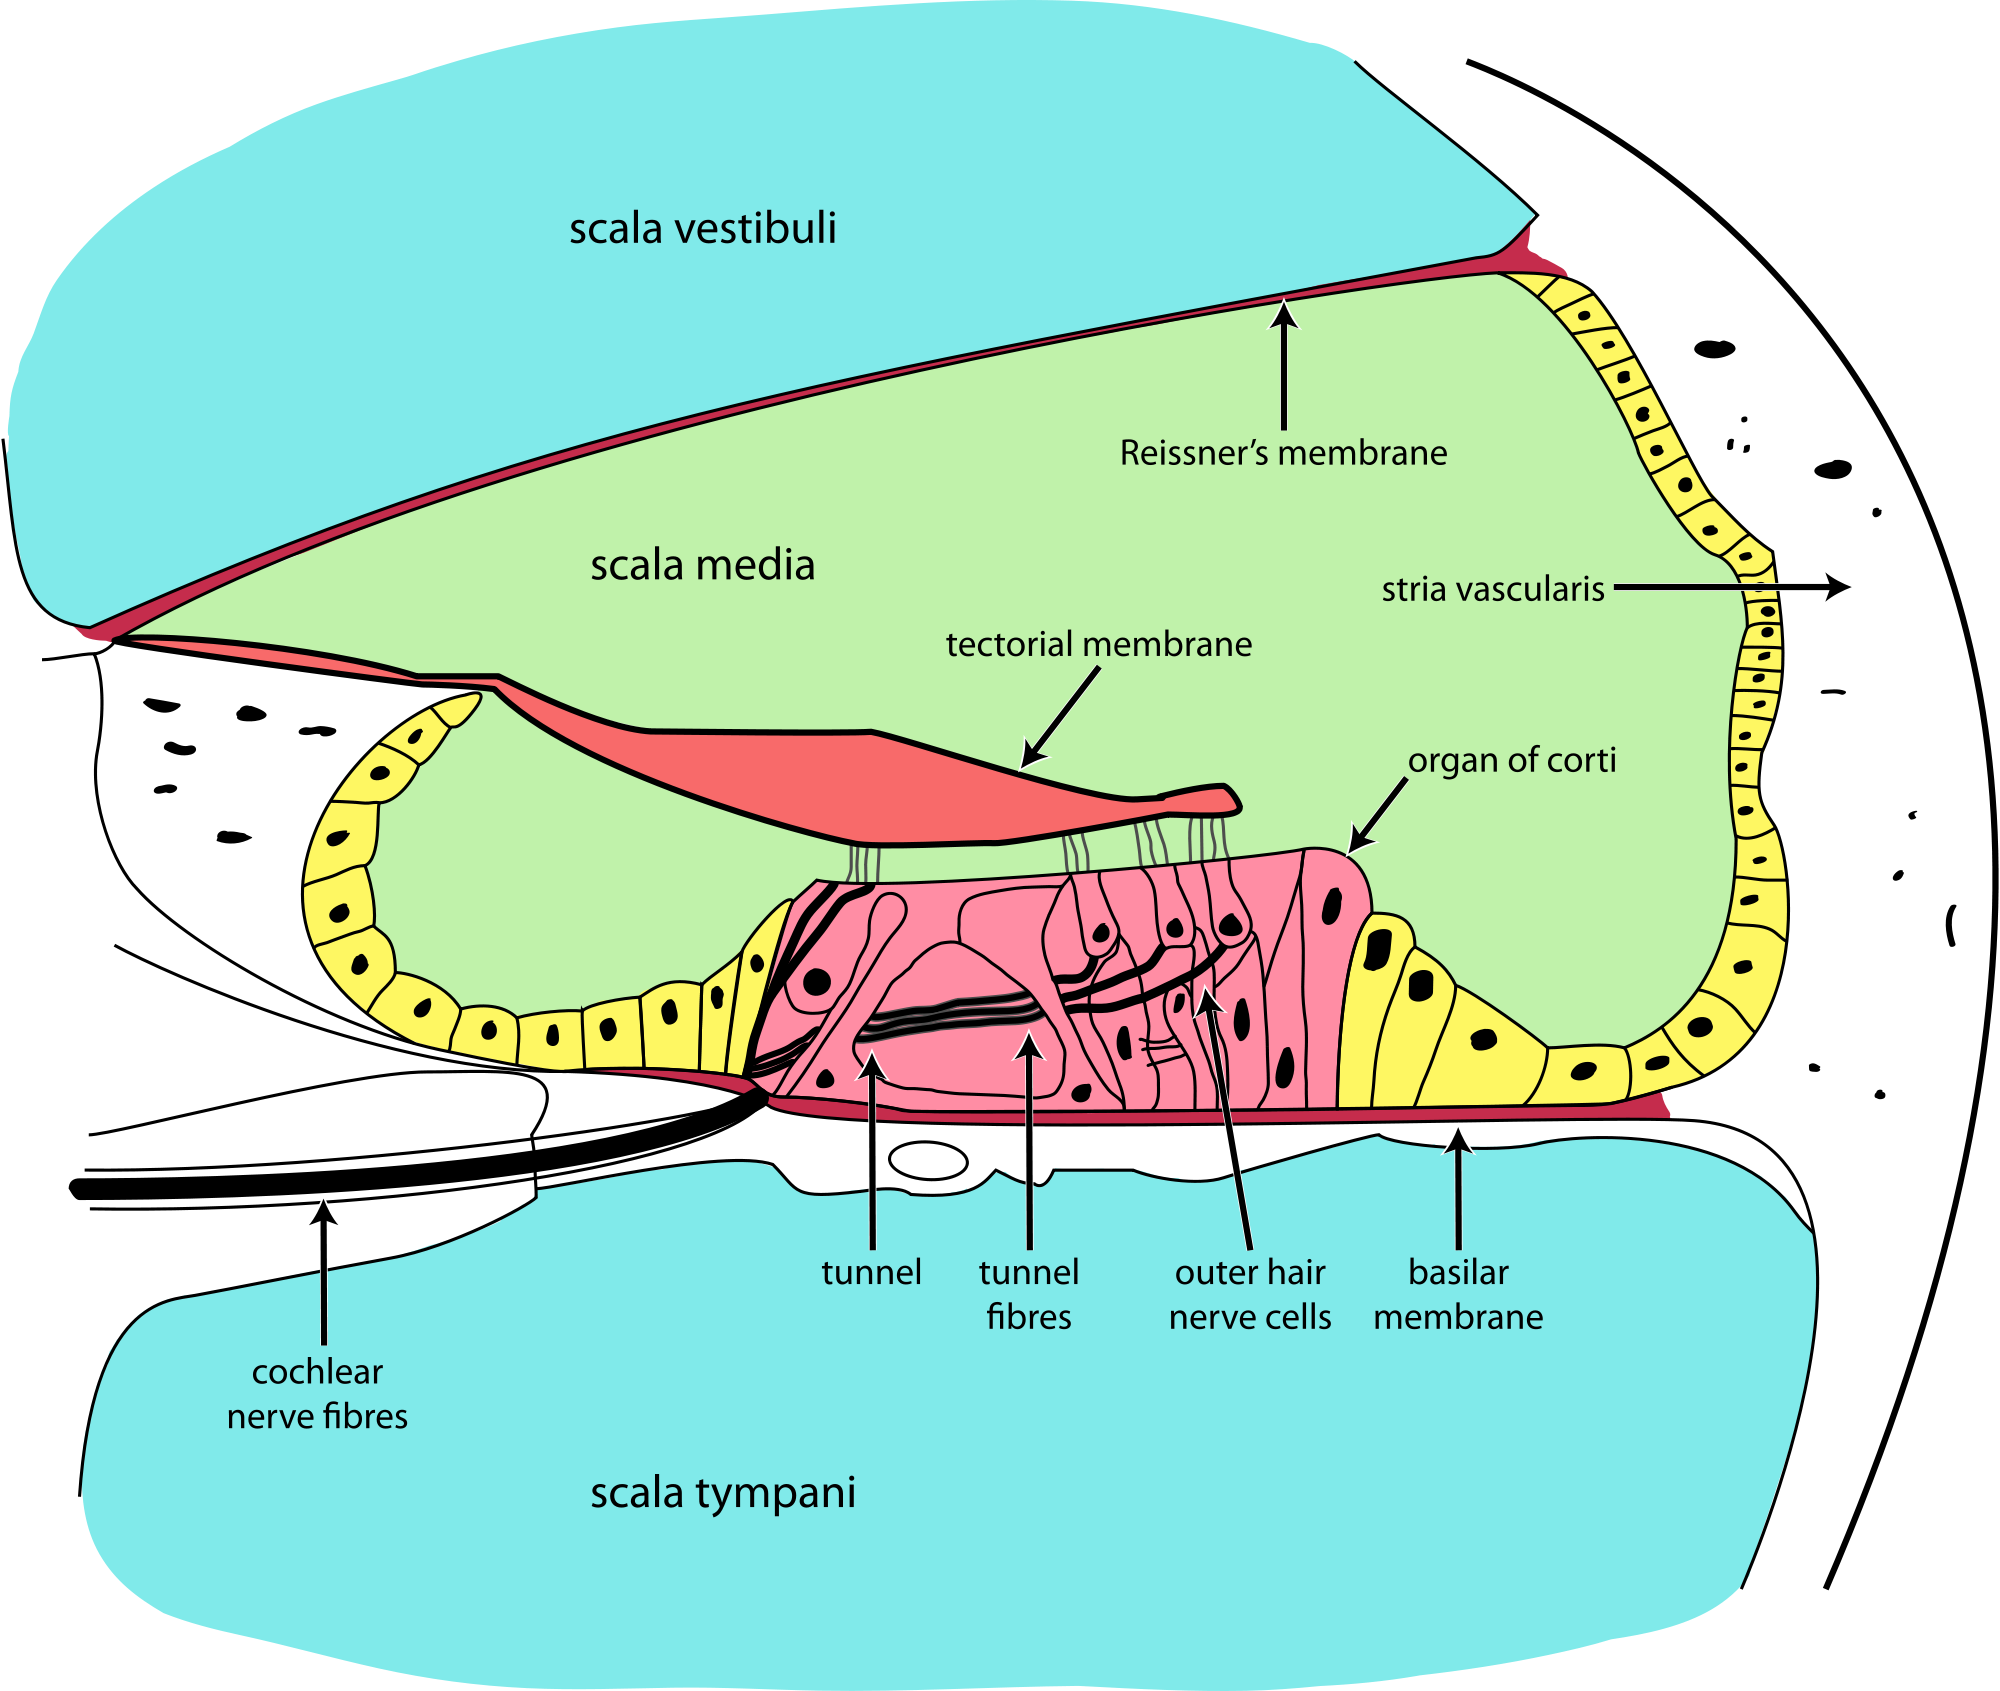
\includegraphics[width=0.85\textwidth]{Images/Background/cochlea_big.png}
      \caption{A schematic of tissues in the cochlea.}
      \label{fig:cochlea}
\end{figure}

A tissue of particular interest in the cochlea is the tectorial membrane, which is in direct contact with the hair cells, as shown in Figure \ref{fig:cochlea}. This tissue's proximity to the sensory cells, and its interesting mechanical properties, including frequency-sensitive acoustic wave propagation, suggest that it could play an active role in auditory frequency discrimination and motion amplification. \cite{Ghaffari2010}

%However, as it is almost entirely water, it is very difficult to image with conventional imaging techniques. \cite{needcitation}

A technique known as optical coherence tomography allows three-dimensional imaging into and through cochlear tissues such as the tectorial membrane, by making use of the auto-correlation properties of temporally incoherent light. This technique can image deeper into tissues than other three-dimensional imaging methods such as confocal microscopy. Furthermore, by measuring the doppler frequency shift of scattered light, OCT allows for measurement of motion, both constant and periodic. \cite{DrexlerBook}

The Micromechanics Group at RLE currently uses a doppler optical coherence microscopy, or DOCM (a subset of doppler optical coherence tomography, or DOCT) system to image the mammalian cochlea and acquire data about the mechanical motions of tissues. This system was developed by former student Stanley Hong, and as of such, will be referred to as the Hong system. \cite{hong}

The Hong system is designed around free space optics that have been carefully aligned and positioned on an optics table. This design has several disadvantages, chiefly that it is difficult and time consuming to align with the animal that is being imaged. This process takes significant time, due to the need to move the animal precisely under the DOCT objective, and the need to align the cochlea with the fixed optical axis of the DOCT system.

The system described in this thesis, while similar in many ways to the existing DOCT system, primarily uses fiber optic (FO) coupled components. Therefore, it will be hereafter referred to as the FO-DOCM system. Fiber optics can be more compact and mobile than free space optical components.. Additionally, the objective used for imaging the actual tissue is mounted on a custom designed mechanical apparatus that allows for an adjustable angle optical axis and easy repositioning, to work with the researcher and research animal, rather than forcing the animal to conform to the optical system. These improvements should significantly improve the workflow of other researchers in the Micromechanics Group.

Additionally, the FO-DOCM system uses a longer wavelength of light than the Hong system, 1310 nm IR instead of 800 nm IR. While this has some disadvantages in terms of axial resolution capability, as discussed in Section \ref{sec:principles_oct}, this wavelength also has several advantages. It is a commonly used wavelength for communication applications, and therefore many optical components are designed for compatibility in this region. More importantly, 1310 nm has significantly reduced scattering through bone tissue, therefore allowing for greater transmission and penetration. This has the potential to obviate the current need to image through either the cochlear round window or a hole cut in the cochlear apex. \cite{Sandell2011} \cite{Bashkatov2006}

\section{Principle of operation of time domain OCT}
\label{sec:principles_oct}

% \begin{figure}[h!]
% \centering
% 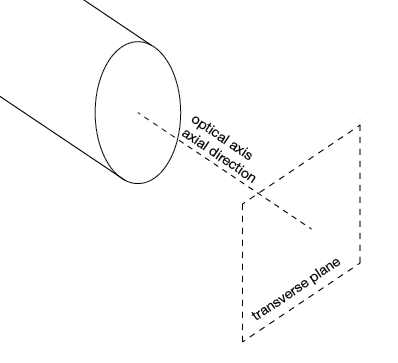
\includegraphics[width=0.4\textwidth]{Images/Background/axes.png}
% \caption{Definition of axes.\label{fig:axis_def}}
% \end{figure}

Throughout this document, the coordinate axis parallel to the direction of light emission from the objective shall be referred to as the ``axial'' direction, or ``z'' axis. The plane perpendicular to this axis is known as the ``transverse'' plane, or, sometimes, the ``x'' and ``y'' axes. %A diagram of this definition is shown in Figure~\ref{fig:axis_def}.

\begin{figure}[h!]
  \centering
    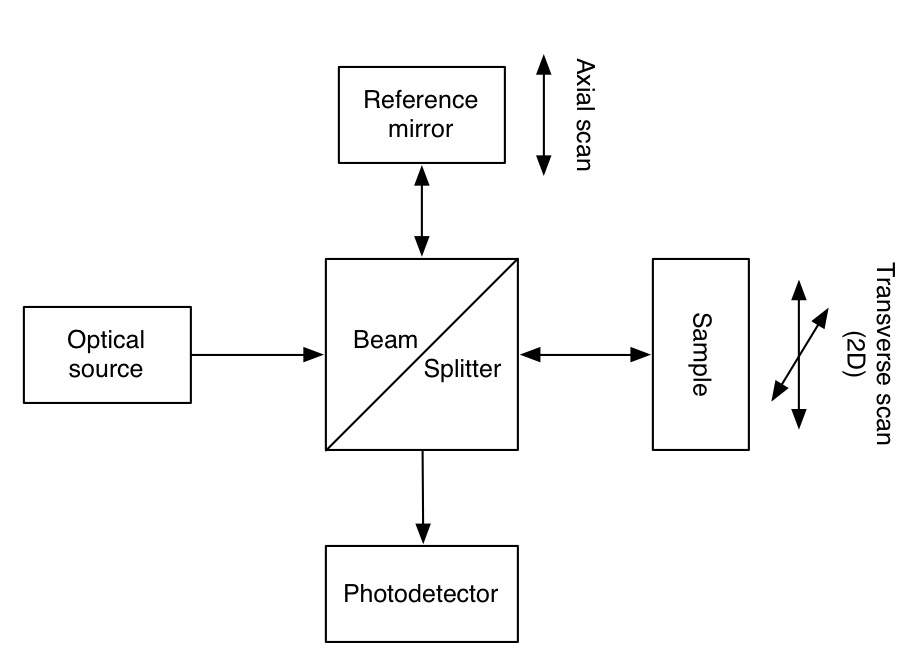
\includegraphics[width=0.75\textwidth]{Images/Background/basic_oct_2.png}
      \caption{Block diagram of a simplified OCT system.\label{fig:basic_oct}}
\end{figure}

OCT functions by utilizing the principle of the Michelson interferometer. A block diagram of a significantly simplified OCT system is shown in Figure~\ref{fig:basic_oct}. Light is split into two beams. One is reflected from a mirror, the other is scattered from a biological sample. The light is then recombined and the intensity measured by a photodetector. When the optical path lengths of the two beams are closely matched, an interference pattern may be observed. By using temporally incoherent (broadband) light, the interference pattern is capable of absolute localization, as will now be shown.

The electric field from a temporally incoherent source can be modeled accurately as a wide-sense stationary random process with a power spectral density corresponding to the optical spectrum of the source. \cite{bouma} In the case where the scattering sample is replaced by a reflecting mirror, the mathematical analysis may be simplified greatly by assuming that the system is analyzing the interference of this random process with itself, delayed by the optical path length difference. From this, we show that interference is the same as autocorrelation, and make use of the Wiener-Khinchin theorem. This derivation follows closely that of Fercher et. al. \cite{fercher}

The intensity of light with analytic (complex) amplitude $V(t)$ is defined as:

\begin{equation}
I(t) = |V(t)|^2 = V^*(t)V(t)
\end{equation}

In an OCT system, the light from a reference path is combined with the light from a sample path after some delay. This may be expressed as:

\begin{equation}
V_D(t; \Delta t) = V_S(t) + V_R(t + \Delta t)
\end{equation}

As measuring instantaneous electric field amplitude is impossible, only the ensemble averages of intensity are of interest. This gives the following result, where $\Gamma_{XY}$ represents the cross correlation between two random processes $X$ and $Y$.

\begin{equation}
\begin{aligned}
\bar{I}_D(\Delta t) & =  \langle I_D(t; \Delta t) \rangle \\
& =  \langle V^*_D(t; \Delta t) V_D(t; \Delta t) \rangle \\
& =  \langle I_S(t) \rangle + \langle I_R(t) \rangle + 2 \Re \{\Gamma_{SR} (\Delta t) \}
\end{aligned}
\end{equation}

$\Delta t$, the time delay between the two signals, is proportional to the path length difference between the two beams, and may be calculated simply as $\Delta t = \Delta z / c$. When both sample and reference paths are illuminated from the same light source, the cross correlation function above simplifies into an autocorrelation function of the light source. From here, the Wiener-Khinchin theorem can be applied, which states that the autocorrelation function of a wide-sense stationary random process is related to the process power spectral density by a Fourier transform.

\begin{equation}
\Gamma_{XX}(\tau) = 2 \int_{0}^\infty S_{XX}(f) \exp(2 \pi j \tau f) \,df
\end{equation}

Therefore, the axial resolution in an OCT system is limited by the spectral properties of the light source. Given a source of center wavelength $\lambda_0$ and FWHM bandwidth $\Delta \lambda$, if a Gaussian PSD is assumed, we may find the width of the autocorrelation function, and therefore the axial resolution. \cite{fercher}

\begin{equation} \label{eq:ares}
\delta_z = l_c = \frac{2 \ln{2}}{\pi} \frac{\lambda_0^2}{\Delta \lambda}
\end{equation}

This is just the envelope of the autocorrelation function, however. The autocorrelation function also has a periodic interference component. This is because the PSD $S_{XX}$ in Equation~\ref{eq:ares} is not centered on a frequency of 0, but instead of the central optical frequency of the source. In the spatial domain, this represents itself as a carrier wave modulating the autocorrelation envelope, with a period of one wavelength. The frequency in time of this carrier as captured by the photodetector is therefore dependent both on the wavelength of the light source, $\lambda_0$, and the speed of the axial scan, $v_s$. Note the factor of two that results from the fact that changing the length of the reference path by a distance $\Delta x$ changes the optical path length by $ 2 \Delta x$. \cite{fercher}

\begin{equation} \label{eq:carrier}
f_{mod} = 2 v_s / \lambda_0
\end{equation}

The transverse resolution limit is the standard diffraction limit for a lens, but, depending on the quality of the objective lens optics, this may not be achievable. In general, diffraction through a circular aperture creates an Airy distribution of light, with size dependent on the diameter of the aperture and its distance from the image. These two distances are combined into the numeric aperture (NA), which in the paraxial approximation is $\approx D/(2f)$, where $f$ is the distance to the image, and $D$ is the aperture diameter. The FWHM size of the diffraction limited Airy disc is given as follows. \cite{hecht}

\begin{equation} \label{eq:tres}
\delta_x = 0.51 \frac{\lambda_0}{\mathrm{NA}}
\end{equation}

\section{Heterodyne OCT with acousto-optic modulators}

As derived in the previous section, the frequency of the carrier is dependent on the speed of the z-axis motion. For typical cases, this is on the order of 1 KHz. If the speed of the scan is variable, this carrier is inconsistent, and if the scan stops at a particular point, the frequency is near zero (non-zero only due to spurious mechanical vibration).

In some cases, such as when phase recovery is necessary, as is the case for the FO-DOCM system, it is desirable to have a higher carrier frequency, or a carrier frequency that is independent of the speed of the z-axis scan. This can also be useful for cases where the z speed is zero, as in en-face OCT. One way to accomplish is through the use of acousto-optic modulators, or Bragg cells, as an optical heterodyne. \cite{bouma} \cite{hitzenberger}

\subsection{Principle of operation of acousto optic modulators}

\begin{figure}[h!]
\centering
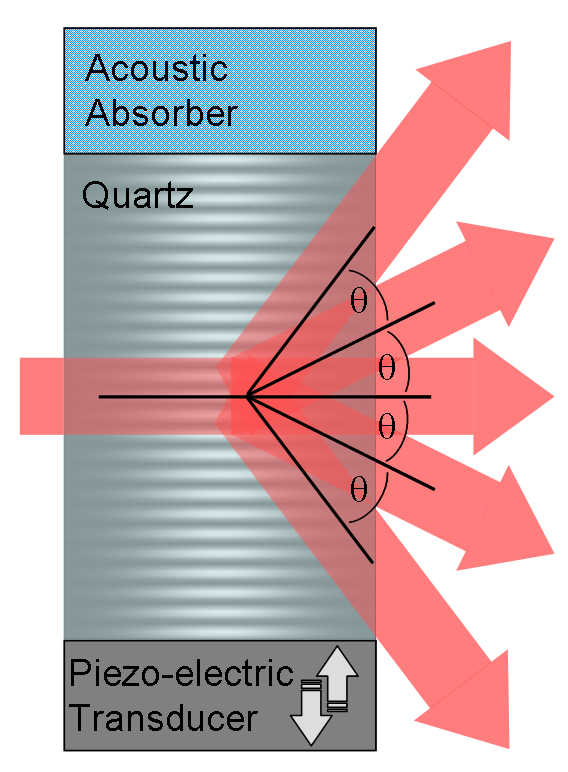
\includegraphics[width=0.3\textwidth]{Images/Background/aom.png}
\caption[Light scatters off of acoustic wavefronts in an acousto-optic modulator.]{Light scatters off of acoustic wavefronts in the quartz crystal of an acousto-optic modulator. As it scatters, it changes both frequency and angle.}
\end{figure}

Acousto-optic modulators (AOMs) are crystals, typically quartz, that use the acousto-optic effect to shift the frequency of light. A transducer establishes an acoustic standing wave at RF frequencies inside the crystal. Acoustic compression waves in the crystal can be modeled as gradients in the refractive index. Light incident upon these refractive index gradients will be scattered, changing its angle and its frequency. Momentum conservation of the scattered light requires the following condition to be satisfied. \cite{haus}

\begin{equation}
\mathbf{k}_{\mathrm{sound}} + \mathbf{k}_{\mathrm{incident}} = \mathbf{k}_{\mathrm{diffracted}}
\end{equation}

This can be solved to give a condition on the angle in the case where $\mathbf{k}_i$ is normal to $\mathbf{k}_s$, where $\lambda$ is the optical wavelength and $\Lambda$ is the acoustic wavelength. A small angle approximation is applied as it is assumed that $|\mathbf{k}_i| \gg |\mathbf{k}_s|$.

\begin{equation} 
\sin{\theta} \approx \frac{|\mathbf{k}_s|}{|\mathbf{k}_i|} = \frac{\lambda}{n\Lambda}
\end{equation}

In some crystals, higher order diffraction angles occur, however, it is difficult to achieve high modulation efficiencies, and they are not of significant interest to this research.

% \begin{figure}[h!]
% \centering
% 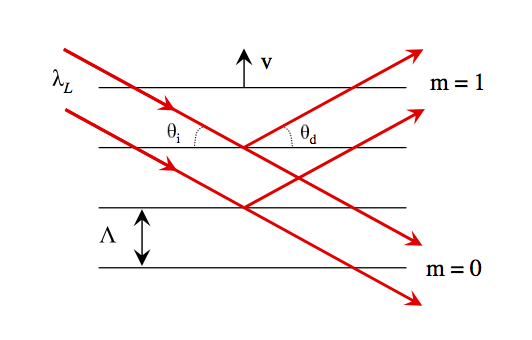
\includegraphics[width=0.5\textwidth]{Images/Background/aom_scattering.png}
% \caption{Light scattering off of acoustic wavefronts in an acousto-optic modulator.}
% \end{figure}

% Scattered light interferes constructively when the following condition is met.

% \begin{equation} \label{eq:constructive_interference}
% n \lambda_L = \Lambda (\sin{\theta_i} + \sin{\theta_d})
% \end{equation}

% Conservation of momentum requires that $\theta_i = \theta_d$, which simplifies the constructive interference condition to:

% \begin{equation}
% n \lambda_L = 2 \Lambda \sin{\theta_d}
% \end{equation}

Energy conservation further requires that the frequency of scattered light be shifted by $F$, the acoustic wave frequency. \cite{haus} This frequency shift is what makes an AOM of practical interest for optical heterodyning.

\subsection{Generating a carrier wave with AOMs}
\label{sec:aom_carrier}

Even with an imprecise or drifting optical center frequency, the precise shift frequency induced by an AOM can be used to generate an extremely stable optical interference signal. \cite{hitzenberger}

The instantaneous complex electric field for a monochromatic plane wave in a particular location may be written for two different frequencies as

\begin{align}
E_a(t) & = E_a \exp{(2 \pi ft j)} \\
E_b(t) & = E_b \exp{(2 \pi (f + F)t j)}
\end{align}

The interference between these two fields creates a beat frequency, with the optical frequency amplitude modulated by the slower RF frequency $F$.

\begin{align}
E_a(t) + E_b(t) = & E_a \exp{(2 \pi ftj)} + E_b \exp{(2 \pi (f + F)t j)} \\
= & E_a \exp{(2 \pi ftj)} + E_b (\exp{(2 \pi ftj)} \exp{(2 \pi Ftj)}) \\
= & E_a \exp{(2 \pi ftj)} (1 + \frac{E_b}{E_a} \exp{(2 \pi Ftj)}) \\
= & E_a(t) (1 + \frac{E_b}{E_a} \exp{(2 \pi Ftj)})
\end{align}

The RF frequency $F$ used to drive the AOMs is typically on the order of 40-200 MHz. For many applications, this is a higher carrier frequency than desired. In this case, it is possible to use two AOMs to generate an even lower frequency carrier, by driving them at slightly different RF frequencies.

\begin{align}
E_a(t) & = E_a \exp{(2 \pi t j (f + F_1))} \\
E_b(t) & = E_b \exp{(2 \pi t j (f + F_2))}
\end{align}

It can be seen via an identical simplification to the above that the combination of these electric field amplitudes creates a carrier wave with frequency equal to the absolute value of $F_1 - F_2$.

\section{Doppler OCT with AOMs}
\label{sec:doppler_aom}

%% more equations/background

Light scattering from moving particles induces a change in the frequency of scattered light, due to the Doppler effect. This change in frequency can be expressed as follows, where $\alpha$ is the angle between the direction of light propagation and the scattered light detector, $\beta$ is the angle between the direction of motion of the media and the direction of light propagation, and $v(t)$ is the instantaneous velocity of the sample. \cite{hurst}

%Because the speed of scattering media will always be much smaller than the speed of the light, the change in frequency caused by the Doppler effect is:

\begin{equation} \Delta f = 2 \frac{v(t)}{c} f_0 \cos{(\beta)} \sin{(\frac{\alpha}{2})} \end{equation}

In the FO-DOCM apparatus, only light that is scattered backwards can be detected, so $\alpha$ is assumed to be $\pi$ radians. The direction of motion is assumed to be in the direction of light propagation for simplicity, so that $\beta = 0$. The equation then simplifies to the following expression for the new instantaneous frequency change.

\begin{equation} \Delta f(t) = 2 \frac{v(t)}{c} f_0 \end{equation}

Integrating the instantaneous frequency gives the phase as follows, where $d(t)$ is the instantaneous sample displacement, the integral of the sample velocity.

\begin{align}
\phi(t) - \phi(0) & = \int_0^{t} 2 \pi f(t) \mathrm{d}t \\
& = 2 \pi \int_0^t f_0 (1 + 2 \frac{v(t)}{c}) \mathrm{d}t \\
& = 2 \pi \left( f_0 t + 2 \frac{d(t)}{c} \right)
\end{align}

The instantaneous electric field amplitudes from Section~\ref{sec:aom_carrier}, $E_a$ and $E_b$, may be written as follows. $E_a$ has been scattered from media moving with the velocity $v(t)$, while $E_b$ has not, representing the sample and reference paths in the OCT system.

\begin{align}
E_a(t) & = E_a \exp{\left(2 \pi j (f + F_1) \left( t + 2 \frac{d(t)}{c}\right) \right)}  \\
E_b(t) & = E_b \exp{(2 \pi t j (f + F_2))}
\end{align}

The electric field at the detector is the sum of the two electric field amplitudes.

\begin{dmath}
E_b(t) + E_a(t) = E_a \exp{(2 \pi t j (f + F_1))}\left(\exp{\left(2 \pi j \frac{2 d(t)}{c}(f + F_1)\right)} + \frac{E_b}{E_a} \exp{(2 \pi t j (F_2 - F_1))}\right)
\end{dmath}

This equation can be simplified slightly by substituting two new symbols for the modified optical frequency, $f' = f + F_1$ and RF frequency difference, $\Delta F = F_1 - F_2$.

\begin{dmath}
E_b(t) + E_a(t) = E_a \exp{(2 \pi t j f')}\left(\exp{\left(2 \pi j f' \frac{ 2 d(t)}{c}\right)} + \frac{E_b}{E_a} \exp{(-2 \pi t j \Delta F)}\right)
\end{dmath}

The instantaneous light intensity is equivalent to the absolute value of the instantaneous electric field amplitude squared.

% \begin{dmath}
% I(t) = E_a^2 \left(1 + \frac{E_b^2}{E_a^2} + 2 \frac{E_b}{E_a} \cos{\left(2 \pi t \left(\Delta F + f' \left( \frac{2 A_o \cos{\omega t}}{c} \right) \right)\right)} \right)
% \end{dmath}

\begin{dmath}
I(t) = E_a^2 + E_b^2 + 2 E_b E_a \cos{ 2 \pi \left(t \Delta F + f' \frac{2 d(t)}{c}   \right)}
\end{dmath}

The result of the frequency shift induced by the motion of the media can clearly be seen in the instantaneous phase of the intensity oscillation.

\begin{dmath}
\label{eq:phase_aom_doppler}
\phi(t) = 2 \pi \left(t \Delta F + f' \frac{2 d(t)}{c}   \right)
\end{dmath}

This is equivalent to phase modulation, with the periodic change in phase of:

\begin{equation}
2 \pi f' \left( \frac{2 d(t)}{c} \right)
\end{equation}

This oscillation can be extracted from the captured signal using the Hilbert transform, as discussed in Section \ref{sec:sigproc_mo_anal}. While this derivation assumed perfectly monochromatic light sources, as would be the case in an ideal laser interferometer, the general result extends to the non-monochromatic random signals used in Section~\ref{sec:principles_oct}.

\section{Signal processing}

%% signal processing figure

\begin{figure}[h!]
  \centering
  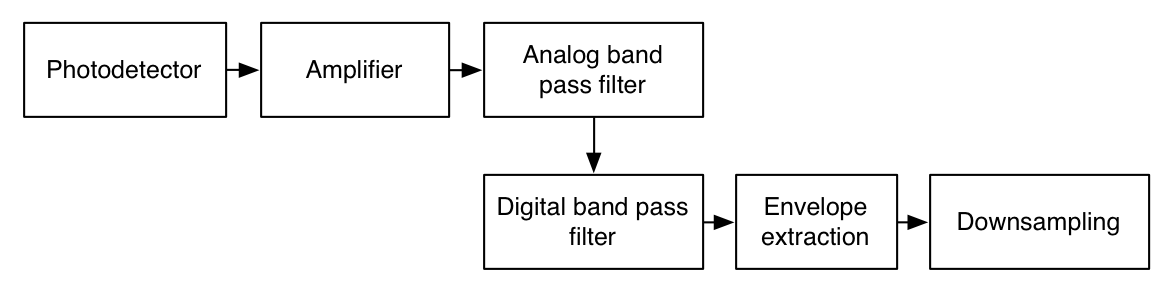
\includegraphics[width=1.0\textwidth]{Images/background/basic_dsp.png}
% \begin{tikzpicture}[node distance = 2cm, auto]
%     % Place nodes
%     \node [block] (bpf) {Analog band pass filter and preamplifier};
%     \node [block, left of=bpf, node distance=3cm] (pd) {Photodiode};
%     \node [block, right of=bpf, node distance=3cm] (adc) {Analog to digital converter};
%     \node [block, below of=adc, node distance=3cm] (dbpf) {Digital band pass filter};
%     \node [block, right of=dbpf, node distance=3cm] (hilb) {Hilbert transform envelope extraction};
%     \node [block, right of=hilb, node distance=3cm] (ds) {Downsampling};
%     % Draw edges
%     \path [line] (pd) -- (bpf);
%     \path [line] (bpf) -- (adc);
%     \path [line] (adc) -- (dbpf);
%     \path [line] (dbpf) -- (hilb);
%     \path [line] (hilb) -- (ds);
% \end{tikzpicture}
\caption[Basic OCT signal processing chain.]{Basic OCT signal processing chain. The bandpass filter is centered around the carrier frequency from equation \ref{eq:carrier}. The demodulator either can be as straightforward as an envelope follower or a Hilbert transform based analytic continuation.}
\end{figure}

After detection and amplification, but prior to analog-to-digital conversion, analog bandpass filters select for the carrier frequency and its sidebands.

The Hilbert transform can be used to extract the envelope from the modulated carrier signal. Given a signal of the form

\begin{equation}
x(t) = A(t)\cos{(\omega t)}
\end{equation}

the Hilbert transform can generate the approximate quadrature component, given by

\begin{equation}
H(x(t)) \approx A(t) \sin{(\omega t)}
\end{equation}

It can therefore be seen that the envelope component of the signal can be calculated quite easily. \cite{oppenheim}

\begin{equation}
A(t) \approx \sqrt{(x(t))^2 + H(x(t))^2}
\end{equation}

The envelope, which does need the high sampling rate previously required in order to capture the carrier frequency, can then be low pass filtered and decimated to the resolution required by the imaging application.

\subsection{Analyzing motion}
\label{sec:sigproc_mo_anal}

%As the reference signal $V_{ref}$ is at exactly half the frequency of the captured heterodyne signal $V_{het}$, the following equation gives the instantaneous difference in phase.

As we showed in Section \ref{sec:doppler_aom}, the phase of the amplitude of light scattered from media moving periodically, which we will refer to as the heterodyne signal, $V_{\mathrm{het}}$, can be expressed as follows.

\begin{equation}
\phi_{\mathrm{het}}(t) = 2 \pi \left(t \Delta F + f'  \frac{2 d(t)}{c}    \right) 
\end{equation}

We also must capture a reference signal, notated as $V_{\mathrm{ref}}$, which is the difference between the two RF drive frequencies. This frequency difference is exactly half the carrier frequency of the heterodyne signal, so its phase may be written as:

\begin{equation}
\phi_{\mathrm{ref}}(t) = 2 \pi t \frac{\Delta F}{2}
\end{equation}

The instantaneous phase of an arbitrary signal may be estimated as follows, where $H$ is the Hilbert transform also discussed in Section \ref{sec:aom_carrier}.

\begin{equation}
\phi(t) \approx \tan^{-1} \left( \frac{H(x)(t)}{x(t)} \right)
\end{equation}

Therefore, the instantaneous phase difference between the heterodyne signal and the reference signal may be written as:

\begin{equation}
\phi_{\mathrm{dif}}(t) \approx \tan^{-1}\left( \frac{H(V_{\mathrm{het}})(t)}{V_{\mathrm{het}}(t)} \right) - 2\tan^{-1}\left( \frac{H(V_{\mathrm{ref}})(t)}{V_{\mathrm{ref}}(t)} \right)
\end{equation}

Substituting in from Equation \ref{eq:phase_aom_doppler}, with $c$ replaced by $c/n$ to account for the refractive index of the media.

\begin{equation}
\phi_{\mathrm{dif}}(t) = \phi_{\mathrm{het}}(t) - 2 \phi_{\mathrm{ref}}(t) = 2 \pi f' \left( \frac{2 d(t)}{c/n} \right)
\end{equation}

Because the RF frequency $F_1 << f$, the optical frequency, we can approximate $f' = f + F_1 \approx f$, and simplify the equation above. The equation can be made simpler still by expressing the optical frequency as a wavenumber.

\begin{equation}
\phi_{\mathrm{dif}}(t) = 2 \pi t f'  \left( \frac{2 d(t)}{c/n} \right) \approx 2 k n d(t)
\end{equation}

Consequently, the periodic displacement of the sample, $d(t)$ may be calculated.

\begin{equation} d(t)  \approx \frac{1}{2kn} \phi_{\mathrm{dif}}(t) \\
%&  \approx \frac{1}{2kn} \left( \tan^{-1}\left( \frac{H(V_{\mathrm{het}})(t)}{V_{\mathrm{het}}(t)} \right) - 2\tan^{-1}\left( \frac{H(V_{\mathrm{ref}})(t)}{V_{\mathrm{ref}}(t)} \right) \right)
\end{equation}

\section{Related work}

Since the 1960s, interferometry with laser light has been used to measure vibration in the cochlea. Early laser doppler interferometer experiments required the placement of reflective beads to isolate tissues of interest, however, these can influence the mechanical properties of the cochlea. \cite{Nuttall2012} Recent methods involving laser doppler interferometry have had success in measuring vibrations as small as 30 picometers without beads, but also require a parallel system, such as confocal microscopy, in order to produce an image of the tissues. Furthermore, laser interferometers are highly coherent, so without reflective beads, vibration measurements have a depth seperation determined primarily by the beam divergence angle. \cite{Jacob2009} \cite{Ren2002} \cite{Ren2011} 

Low coherence interferometry, such as OCT, is capable of solving these problems. As mentioned in Section \ref{sec:intro}, this FO-DOCM system is designed to update the previous system used in the Micromechanics Group, designed and constructed by Stanley Hong. The FO-DOCM system is quite similar to Hong's work, but is also different in several ways: the use of fiber optic components rather than free space optics, the use of a longer wavelength source, and, most importantly, the revised alignment and positioning apparatus. Additionally, the FO-DOCM system allows for continuous scanning of lines in an image, rather than point-by-point pixel acquisition. \cite{hong}

\paragraph{Other time-domain doppler OCT systems} The use of acousto-optic modulators is not essential for doppler OCT, and systems similar to the FO-DOCM system have been constructed without them. However, without a reference signal to use in extracting phase modulation information, the system responds to vibration amplitude in a very non-linear way. Furthermore, because vibrations are not modulated to higher frequencies by the heterodyne carrier, more interference at low frequencies, from mechanical vibrations and other $1/f$ noise, results in a higher noise floor, typically on the order of 30 pm/Hz$^{0.5}$. \cite{Choudhury2006}

\paragraph{Spectral-domain doppler OCT systems} While the FO-DOCM project uses time-domain doppler OCT, work has also been done in the field of spectral domain doppler OCT.  In order to detect motion, a spectral-domain OCT system must be sensitive to changes in optical phase. This is unlike the system described in this thesis, which may be constructed from standard single mode optical fibers, despite the randomization of phase that they induce. Spectral-domain doppler OCT systems have achieved results with an axial resolution of 13 microns and a motion detection noise floor of 300 pm. It is thought that a time domain approach can result in higher resolution motion measurements, as a monolithic photodiodes have better noise equivalent power then a CCD line camera with a diffraction grating. Furthermore, the sampling rate of a CCD sensor is very limited compared to a photodiode, restricting the speed of phase acquisition. However, the use of a time-domain system adds the considerable expense of requiring physical motion to scan the z-axis, resulting in significantly slower image acquisition. \cite{Choudhury2011} \cite{Subhash2012}

\paragraph{Trans-bone imaging} Doppler OCT has been previously used with some success for measuring vibrations of cochlear tissues through bone. With a 935 nm center wavelength, motion inside an {\em in vivo} mouse cochlea was measured, with an noise floor of approximately 100 pm/Hz$^{0.5}$. \cite{Gao2013} It is suspected that a 1310 nm center wavelength, as used in the FO-DOCM system, will be even more effective at penetrating bony tissue. \cite{Sandell2011} \cite{Bashkatov2006}

\paragraph{Microangiography} Doppler OCT is not restricted to measuring periodic vibrations -- one of its first applications was for angiography, measuring the velocity of blood flow inside tissue. Current techniques with doppler optical microangiography are capable of isolating and measuring bloodflow in a single vessel over time. While low frequency motion measurements such as constant motion hae a significantly higher noise floor for measurement, blood flow velocity amplitudes are typically much greater than vibrational amplitudes. \cite{Dziennis2012}

%\subsection{Positioning and GRIN lens}

\paragraph{Minituarization of OCT apparatus} One of the advantages of the FO-DOCM system to the Micromechanics Group is its smaller size, so this work may be seen as continuing the active effort of minimizing the size of the OCT apparatus. Research in this area includes the creation of a miniature swept frequency laser source for OCT imaging, which could enable a higher axial resolution in a smaller form factor. \cite{Goldberg2009} GRIN lenses, in addition to near diffraction limited optical performance, also have a significant size advantage, and have also been used in previous research as endoscopic probes for OCT. \cite{Xie2006}

% talk about uniqueness of our mechanical apparatus?

% small size is relevant here???


% ====================================

% 

% %Why time domain? This differentiates our work? Can I spin it positively?

% \cite{Choudhury2011}  % The FO-DOCM system is shown to be competitive with these results. \cite{Choudhury2011} \cite{Subhash2012}


% Also of interest in the development of this system, and still a developing technique, is the use of algorithms and more sophisticated signal processing techniques to improve the image quality and resolution ability of captured OCT data. Of significant interest is the possibility of correcting for dispersive effects caused by the propogation of light through the sample media. \cite{Xie2005} \cite{DrexlerBook} These techniques could also potentially be used to correct for dispersion caused by fiber length mismatch between the reference and sample paths, as discussed in Section~\ref{sec:reference_path}.

\paragraph{} Overall, the FO-DOCM system designed and constructed in this thesis builds on previous work and ideas in optical coherence tomography to develop an apparatus that satisfies the unique set of requirements of the Micromechanics Group.